\chapter{Implementation des Systems}
\label{Implementation_des_Systems}
Im Folgenden wird die Implementation des Systems erläutert, wobei zu Beginn Arbeitspakete definiert werden, die daraufhin bearbeitet werden. Die Dokumentation der Implementation wird, wo notwendig, mit Auszügen des Sourcecodes erweitert. Der vollständige Sourcecode ist unter \url{https://github.com/astrutz/masterthesis} zu finden, eine Instanz zum Testen liegt unter \url{https://pay2mail.org} vor.

\section{Umwandlung der Anforderungen in Arbeitspakete}
Um die in Kapitel \ref{Definition_von_Nutzeranforderungen} definierten Nutzeranforderungen zu strukturieren und die Entwicklung einzelner Features klar abzugrenzen, werden Arbeitspakete erstellt. Die Arbeitspakete werden so sortiert, dass die Anforderungen mit der höchsten Priorität zu Beginn implementiert werden. Das hat den Vorteil, dass bei fehlenden zeitlichen Ressourcen die wichtigsten Features bereits implementiert sind und Pay2Mail trotzdem nutzbar ist, wenn auch mit kleineren Einschränkungen. Tabelle \ref{tab:arbeitspakete} zeigt die Zuordnung der Anforderungen zu ihren jeweiligen Arbeitspaketen.

\begin{table}[!h]
\centering
\caption[Arbeitspakete der Implementation]{Zuordnung der Anforderungen zu Arbeitspaketen}
\begin{tabular}{|l|l|}
\rowcolor{red!25}
\hline
\textbf{Nutzeranforderung}               & \textbf{Arbeitspaket}            \\ \hline
Einsicht in das Aufkommen des Empfängers & Einsicht in das E-Mail Aufkommen \\ \hline
Priorisierbarkeit mit Gegenwert          & Priorisierung von E-Mails        \\ \hline
Technologisch unabhängige Nutzung        & -                                \\ \hline
Sicherheit der E-Mails und Zahlungen     & -                                \\ \hline
Keine Verlangsamung des E-Mail Prozesses & -                                \\ \hline
Automatische Triage                      & Automatische Triage              \\ \hline
Definition der Bearbeitungsleistung      & Einsicht in das E-Mail Aufkommen \\ \hline
Integrität der E-Mails und Zahlungen     & -                                \\ \hline
Abweichungen der automatischen Triage    & Automatische Triage              \\ \hline
Erreichbarkeit                           & -                                \\ \hline
Koexistenz zu bisherigen Kanälen         & -                                \\ \hline
Intuitive Nutzung                        & -                                \\ \hline
\end{tabular}
\label{tab:arbeitspakete}
\end{table}

\noindent Grundsätzlich werden obligatorische drei Arbeitspakete, sowie ein optionales Arbeitspaket, formuliert. Das erste Paket implementiert die Einsicht in das E-Mail Aufkommen. Hierfür wird das Frontend des Prototyps um Realdaten erweitert. Um Realdaten zu erhalten, werden die notwendige Datenstruktur und das Backend aufgesetzt, welches die E-Mails des MDA abruft. Daraufhin wird das Paket zur Priorisierung von E-Mails implementiert. Dabei wird die Datenstruktur um (simulierte) Zahlungen und die Priorität erweitert, auch hier wird das Frontend des Prototyps weiter verwendet. Die automatische Triage bildet das dritte Arbeitspaket ab, bei welcher eine Erweiterung der Datenbasis um Abweichungen der Triage notwendig wird. Außerdem wird ein Service implementiert, der die eigentliche Triage übernimmt. Das vierte Arbeitspaket ist die Anbindung realer Zahlungsanbieter. Dieser Schritt wurde bewusst ausgelagert, da er die Recherche nach APIs zur Abwicklung von Zahlungen und die Erweiterung der Architektur aus den Abbildungen \ref{fig:Datenmodell} und \ref{fig:Komponentenmodell} miteinbezieht. Dadurch bringt die Anbindung der Zahlungsanbieter eine größere Komplexität mit, die den zeitlichen Rahmen dieser Arbeit übersteigt. Das Arbeitspaket wurde jedoch trotzdem definiert als Ausblick, sowie als mögliches Zusatzfeature, falls die Implementation schneller abgeschlossen wird als vermutet. Andernfalls wird Pay2Mail so vorbereitet, dass die spätere Anbindung eines Zahlungsanbieters mit möglichst wenig Aufwand umsetzbar ist. 

In der Zuordnung in Tabelle \ref{tab:arbeitspakete} ist zu sehen, dass ein Großteil der Nutzeranforderungen nicht in Arbeitspakete überführt wird. Das hängt damit zusammen, dass sie bereits implizit durch die Architektur oder technische Grundvoraussetzungen umgesetzt werden. Die technologisch unabhängige Nutzung ist durch die Implementation als Webseite gegeben. Da die Einbindung mehrerer E-Mails Clients über den zeitlichen Rahmen dieser Arbeit hinausgeht, wird lediglich das Web-Frontend implementiert, welches die einzelnen Clients individuell integrieren können. Die Sicherheit der E-Mails bleibt Aufgabe der Clients, da der Versand weiterhin über sie stattfindet. Die Sicherheit der Zahlungen hingegen wird durch die Nutzung von HTTPS und verschlüsselten Datenbanken gewährleistet. Diese Features gehören zum Standard von Ruby on Rails und müssen daher nicht separat implementiert werden. Damit der E-Mail Prozess nicht verlangsamt wird, wird der Code in der CI/CD Pipeline auf verschiedene Fehlerquellen untersucht, die die Anwendung verlangsamen können, siehe dazu auch Kapitel \ref{Projekt_Setup_und_Einrichtung_einer_CI/CD Pipeline} und Sourcecode \ref{lst:pipeline}. Die Integrität der E-Mails und Zahlungen wird durch die Nutzung eines E-Mail Headers mit UUID sicher gestellt. Da die UUID in der Datenbank zusammen mit anderen Metadaten der E-Mail abgeglichen wird (siehe auch \ref{Datenmodell}), können Zahlungen nicht gefälscht oder wiederverwendet werden. Die Erreichbarkeit wird durch das Hosting bei DigitalOcean sichergestellt, welches bei Serverausfällen oder anderen Fehlern den Inhaber der Anwendung informiert. Die Koexistenz zu bisherigen Kanälen ist durch die Systemarchitektur impliziert, da E-Mails nicht ersetzt, sondern bei Bedarf nur erweitert werden. Die intuitive Nutzung der Anwendung ist eine Anforderungen, die sich nur unzureichend in konkrete Arbeitsschritte formulieren lässt. Stattdessen werden in der Implementation die Grundsätze der Dialoggestaltung nach ISO 9241-110 berücksichtigt, insbesondere \textit{Steuerbarkeit}, \textit{Erwartungskonformität}, \textit{Fehlertoleranz} und \textit{Selbstbeschreibungsfähigkeit} \citep{ISO9241-110}. Ob dies die intuitive Nutzung schlussendlich unterstützt, wird die Nutzerevaluation in Kapitel \ref{Nutzerevaluation_des_Systems} aufzeigen. 

%----------------------------------------------------

\section{Einsicht in das E-Mail Aufkommen}
\label{Einsicht_in_das_E-Mail_Aufkommen}

Das erste Arbeitspaket implementiert zwar die Einsicht des Absenders in das Aufkommen, darüber hinaus werden jedoch auch strukturelle Grundlagen geschaffen und das Datenbankschema umgesetzt. Zu Beginn werden die frontendseitigen Routen erweitert. Im Prototyp war es lediglich möglich mit \texttt{/send} auf die Übersicht des Absenderfrontends zu kommen, während die übergeordnete Route \texttt{/} einen 404-Fehler zurückgab. Zur Vorbereitung auf das später folgende Empfängerfrontend wurde eine Startseite implementiert, die die Möglichkeit bietet auf das Absenderfrontend oder das Empfängerfrontend zu wechseln. Ein entsprechender Screenshot ist in Anhang \ref{fig:screenshot_overview} zu sehen. Zur Trennung der beiden Frontendkomponenten werden zwei Namespaces verwendet, die in \texttt{routes.rb}, zu sehen in Sourcecode \ref{lst:routes}, deklariert werden. Die Namespaces fungieren als logische Klammern um das jeweilige Frontend und grenzen es innerhalb einer Route ab, sodass sich jede absenderbezogene Ressource unter \texttt{/send/*} und jede empfängerbezogene Ressource unter \texttt{/receive/*} befindet. Die Verbindung zwischen Namespace und späterer Route als \texttt{:sender} und \texttt{/send} wird mit dem Gem \texttt{route\_translator} realisiert, welches mehrsprachige Routen, sowie kanonische Benennung von Ressourcen ermöglicht \citep{LLuelles2022}. Der Namespace des Empfängers ist auskommentiert und wird im dritten Arbeitspaket implementiert.

\begin{listing}[!ht]
\inputminted[linenos]{ruby}{Listings/Pkg1/routes.rb}

\caption
    [Deklaration der HTTP-Routen]
    {Deklaration der HTTP-Routen (\texttt{config/routes.rb})}

\label{lst:routes}
\end{listing}

\noindent Zur Speicherung der Prioritäten und des Aufkommens wird das in Kapitel \ref{Datenmodell} konzipierte Datenmodell umgesetzt. Anpassungen der Datenbank werden in Rails stets in Migrationen umgesetzt. Eine Migration beschreibt welche Änderungen an der bestehenden Datenbank gemacht werden, wie Felder portiert werden und was mit Bestandsdaten passiert. Zur Erstellung einer Migration kann die Rails CLI genutzt werden mit dem Befehl \texttt{rails generate migration name\_der\_migration}. Daraufhin wird eine Migrationsdatei erstellt mit einer Funktion \texttt{change}, in welcher verschiedene Datenbankänderungen definiert werden, wie z.B. \texttt{create\_table}, zu sehen in Sourcecode \ref{lst:migration}. In diesem Beispiel wird die Tabelle für das Datenobjekt \texttt{Rule} erstellt mit den zwei Feldern als String. Zusätzlich wird die Assoziation zur \texttt{Inbox} aufgebaut, welche eine 1:n-Beziehung zu \texttt{Rule} hat. Da für solche Assoziationen bereits andere Tabellen vorhanden sein müssen, ist die Reihenfolge der Migrationen relevant. Es können mehrere Migrationen erstellt werden, bevor diese ausgeführt werden. Zur Ausführung wird der Befehl \texttt{rails db:migrate} genutzt. Erkennt Rails, dass es offene Migrationen gibt, kann der Server nicht gestartet werden, bis die Migrationen abgeschlossen sind. Das Datenbankschema wird in der Datei \texttt{schema.db} festgehalten und mit jeder Migration aktualisiert. Zudem werden Validierungen, Constraints und Assoziationen in den jeweiligen Models unter \texttt{app/models} festgehalten. Ebenfalls können Callbacks auf bestimmte Events genutzt werden.

\begin{listing}[!ht]
\inputminted[linenos]{ruby}{Listings/Pkg1/20220923155901_create_rules.rb}

\caption
    [Migration der Tabelle \texttt{Rules}]
    {Erstellung der Datenbanktabelle \texttt{Rules} als Migration (\texttt{db/migrate/20220923155901\_create\_rules.rb})}

\label{lst:migration}
\end{listing}

\noindent Um die Datenbank lauffähig und sicher zu gestalten, sind mehrere Anpassungen am Datenmodell notwendig. Die vorgesehene Beziehung zwischen \texttt{Value} und \texttt{Message} wurde aufgelöst. Zum Einen wird ein Gegenwert hinterlegt, bevor eine Nachricht versendet und somit in der Datenbank erstellt wurde, was eine intiale Beziehung nicht möglich macht. Außerdem verhindert eine Beziehung zwischen Nachricht und Gegenwert die direkte Überprüfung, ob ein Gegenwert zu einer Nachricht besteht und inwieweit die Metadaten der E-Mail übereinstimmen. Daher wird in der \texttt{Message} lediglich der Gegenwert-Header, also die UUID, gespeichert. Der \texttt{Value} enthält ebenfalls die UUID, sowie Metadaten zur E-Mail, wie anfänglich konzipiert. Allerdings ist die Speicherung aller E-Mail Header überflüssig, da bereits mit Versandzeitpunkt, Empfänger und Absender eine eindeutige Zuordnung möglich ist.
Im Datenmodell wurde die Verschlüsselung von Inhalten nicht betrachtet. Um jedoch die Anforderung \textit{Sicherheit der E-Mails und Zahlungen} einzuhalten, ist eine Verschlüsselung notwendig. Mit dem Gem \texttt{bcrypt} wird der Befehl \texttt{encrypts :feldname} hinzugefügt, welcher ausgewählte Datenbankfelder verschlüsselt.

\begin{listing}[!ht]
\inputminted[firstline=16, lastline=27,linenos]{ruby}{Listings/Pkg1/schema.rb}

\caption
    [Auszug: Definition von \texttt{Credentials} im Datenbankschema]
    {Auszug: Definition der Tabelle \texttt{Credentials} im Datenbankschema (\texttt{db/schema.rb})}

\label{lst:credentials}
\end{listing}

\noindent Außerhalb der Absicherung von Inhalten wurde ein wichtiger Bestandteil im Datenmodell ausgelassen. So sind zum Abrufen von E-Mails via IMAP entsprechende Zugangsdaten notwendig, die bisher jedoch nicht konzeptioniert wurden. Daher wird eine neue Tabelle \texttt{Credentials} erzeugt. Diese enthält den Servernamen als String, den Port als Integer, Informationen zu SSL und Authentifizierungstyp als String, sowie Nutzername und Passwort als String, welche jedoch verschlüsselt werden. Zudem wird eine 1:1-Beziehung zwischen \texttt{Recipient} und \texttt{Credential} definiert, wobei ein Credential nur so lange wie der Recipient existiert, sodass keine Anmeldedaten bei der Löschung eines Empfängers bestehen bleiben.

Um die Datenbank mit Nachrichten zu befüllen, wird folgend das Modul zum Abrufen der E-Mails implementiert. Da es noch nicht möglich ist aus dem Frontend Empfänger zu erstellen, werden zu Beginn Beispielnutzer mit realen IMAP-Daten erzeugt und der Datenbank hinzugefügt. Das Aufkommen dieser Nutzer lässt sich in der Testinstanz abrufen, die zugehörigen E-Mail Adressen lauten \\ \texttt{pay2mail-test01@freenet.de} und \texttt{pay2mail-test02@freenet.de}. Zur Umsetzung des Moduls wird \textit{ActiveJob} verwendet. ActiveJob ist ein Bestandteil von Ruby on Rails zur Ausführung von Routinen und Skripten (\textit{Jobs}) in einer Warteschlange. Außerdem ist es möglich Jobs zeitlich per \texttt{crontab} o.ä. zu planen und sie so regelmäßig auszuführen \citep{Hansson2022b}. Der Einstiegspunkt des Jobs ist die Funktion \texttt{perform}, die von Rails selbst oder Gems zur Verwaltung von Jobwarteschlangen angestoßen werden kann. Das Modul, benannt \texttt{EmailLoadJob}, iteriert durch eine Menge an Empfänger, meldet sich für jeden per IMAP beim MDA an, lädt alle ungelesenen E-Mails und speichert sie, falls nötig, in der Datenbank. Ein Auszug des Sourcecodes ist in \ref{lst:job} zu sehen, der vollständige Sourcecode ist in Anhang \ref{lst:job_full} abgebildet. Zur Nutzung des IMAP wird das Gem \textit{Mail} verwendet, welches Ruby-ähnliche Syntax bietet. Die zu iterierende Menge an Empfänger ist abhängig vom Kontext des Jobaufrufs. Daher wurde als reasonable default (siehe \ref{Ruby_on_Rails}) die Menge aller Empfänger gesetzt. So lässt sich der Job im Produktivbetrieb in einem Intervall ausführen und prüft die offenen E-Mails für alle Empfänger im Hintergrund. Außerdem lässt sich eine eigene Menge an Empfängern übergeben, so können beim Aufruf von \texttt{/capacity} die E-Mails eines Empfängers geprüft werden und das reale Aufkommen in Echtzeit dargestellt werden.

\begin{listing}[!ht]
\inputminted[firstline=4, lastline=11,linenos]{ruby}{Listings/Pkg1/email_load_job.rb}

\caption
    [Auszug: Job zum Laden der E-Mails]
    {Auszug: Job zum Laden der E-Mails beim MDN (\texttt{app/jobs/email\_load\_job.rb})}

\label{lst:job}
\end{listing}

\noindent Zur Darstellung des Aufkommens in Echtzeit muss der entsprechende Controller erweitert werden, siehe Sourcecode \ref{lst:capacities_controller_pkg1}. Anfangs wird in der Funktion \texttt{fetch\_recipient} anhand des übergebenen Queryparameters nach einem Empfänger in der Datenbank gesucht. Falls keiner gefunden wird, wird eine 404-Seite angezeigt mit dem Hinweis, dass der entsprechende Empfänger Pay2Mail nicht nutzt. Wird jedoch ein Empfänger gefunden, wird daraufhin der Job zum Laden der E-Mails mit der Empfängeradresse gestartet. Anhand des Empfängers wird der zugehörige Posteingang und die Anzahl der enthaltenen Nachrichten geladen. Da die Nachrichten nur so lange im Posteingang verweilen, bis sie bearbeitet wurden, kann diese Summe genutzt werden. Eine Nachricht gilt als bearbeitet, sobald sie vom Empfänger als gelesen markiert wurde. Diese Mechanik wird in Kapitel \ref{Automatische_Triage} genauer erläutert. Zusätzlich wird die Bearbeitungsleistung des Empfängers aus der Datenbank geladen. Zuletzt wird das voraussichtliche Antwortdatum berechnet, analog zum Vorgehen im Prototypen. Hierbei ist die Berechnung nun aus der View in den Controller ausgelagert worden, um die MVC-Architektur zu wahren. In der View zu \texttt{/capacities} werden die im Controller befüllten Instanzvariablen \texttt{@mails\_count}, \texttt{@editing\_performance} und \texttt{@target\_date} lediglich ausgegeben.

\begin{listing}[!ht]
\inputminted[linenos]{ruby}{Listings/Pkg1/capacities_controller.rb}

\caption
    [Erweiterter Controller für Empfänger-Aufkommen]
    {Erweiterter Controller für Empfänger-Aufkommen mit Realdaten (\texttt{app/controllers/sender/capacities\_controller.rb})}

\label{lst:capacities_controller_pkg1}
\end{listing}

%----------------------------------------------------

\section{Priorisierung von E-Mails}
\label{Priorisierung_von_E-Mails}
Das zweite Arbeitspaket verbindet das zuvor erstellte Datenbankschema mit Realdaten, sodass E-Mails priorisiert werden können. Damit Nutzer sehen können wie viel sie für die Priorisierung an einem bestimmten Tag zahlen müssen, wird die Tabelle auf der Seite \texttt{/send/priority} (vgl. Anhang \ref{fig:screenshot_send/priority}) so angepasst, dass sie das Aufkommen aus der Datenbank anzeigt. Da das Model \texttt{Message} lediglich die UUID, aber nicht den Gegenwert selbst enthält, muss vorher eine entsprechende Verknüpfung aufgebaut werden. Dazu iteriert die Funktion \texttt{with\_value} im Model \texttt{Message}, siehe Sourcecode \ref{lst:message1}, durch eine Menge an Nachrichten und sucht einen entsprechenden \texttt{Value}. Hierbei werden die UUID, die Adressen von Empfänger und Absender, sowie das Versanddatum der E-Mail geprüft. Das Versanddatum wird mit der Erstellungszeit des \texttt{Value}, dem automatisch generierten Feld \texttt{created\_at}, verglichen. Da die Zahlung und das Versenden der E-Mail nicht zeitgleich geschehen, wird eine Karenzzeit von 30 Minuten gegeben, nach welcher eine E-Mail versendet sein muss, um einem Gegenwert zugeordnet werden zu können. Dieses zeitliche Limit ergibt sich aus der Anforderung \textit{Sicherheit der Zahlungen}. Nach der Verknüpfung wird das Feld \texttt{value\_header} mit der Höhe des Gegenwertes überschrieben oder leer gelassen, falls kein Gegenwert-Header vorhanden ist.

\begin{listing}[!ht]
\inputminted[firstline=4, lastline=20,linenos]{ruby}{Listings/Pkg2/message.rb}

\caption
    [Auszug: Verknüpfung der Nachrichten mit ihren Gegenwerten]
    {Auszug: Verknüpfung der Nachrichten mit ihren Gegenwerten (\texttt{app/models/message.rb})}

\label{lst:message1}
\end{listing}

\noindent Um die Nachrichten nach ihren voraussichtlichen Bearbeitungstagen zu gruppieren, müssen sie zuerst sortiert werden. Dafür wird das neu befüllte Feld \texttt{value\_header} verwendet, das die Höhe der Zahlungen enthält. Die Sortierung erfolgt nach diesem Feld, E-Mails, die keinen Gegenwert enthalten, werden rückwärts nach ihrem Versanddatum sortiert. Das bedeutet, dass die Liste zuerst die E-Mails mit absteigendem Gegenwert und dann die E-Mails ohne Gegenwert mit aufsteigendem Versanddatum enthält. So ist sichergestellt, dass zuerst E-Mails mit Gegenwert und danach die ältesten E-Mails ohne Gegenwert bearbeitet werden. Daraufhin werden die E-Mails der jeweiligen Tage gruppiert. Dazu iteriert eine Schleife über die sortierte Liste und fügt jede Nachricht der Gruppe des aktuellen Tages \texttt{current\_group} hinzu. Sobald der Index der Schleife durch die Bearbeitungsleistung des Empfängers teilbar ist, wird die Gruppe der Gesamtmenge hinzugefügt und geleert. Die Teilbarkeit des Index zeigt an, dass eine Gruppe exakt die Größe hat, die vom Empfänger an einem Tag bearbeitet werden kann. Daher wird sie daraufhin der Gesamtmenge hinzugefügt. Diese Gruppierung wird für jede Nachricht wiederholt, wobei die letzte Gruppe unter Umständen weniger Nachrichten enthält, als der Empfänger an einem Tag bearbeitet. Die Gesamtmenge der Gruppierung ist ein Array, das wiederum für jeden Tag ein Array an Nachrichten enthält, das zu bearbeiten ist. Die erste Gruppe in der Gesamtmenge spiegelt die Nachrichten für \textit{Morgen} wieder, die zweite Gruppe spiegelt die Nachrichten für \textit{Übermorgen} wieder usw. Der Algorithmus zur Gruppierung ist in Sourcecode \ref{lst:message2} dargestellt.

\begin{listing}[!ht]
\inputminted[firstline=22, lastline=38,linenos]{ruby}{Listings/Pkg2/message.rb}

\caption
    [Auszug: Gruppierung der Nachrichten nach Gegenwerten]
    {Auszug: Gruppierung der Nachrichten nach Gegenwerten basierend auf der Bearbeitungsleistung des Empfängers (\texttt{app/models/message.rb})}

\label{lst:message2}
\end{listing}

\noindent Die gruppierten Nachrichten ermöglichen es nun die Tabelle der Priorisierung zu befüllen. Dazu wird in der View durch die gruppierten Nachrichten \texttt{@messages\_grouped} iteriert und für jede Gruppe eine neue Zeile in der Tabelle erzeugt, siehe Sourcecode \ref{lst:capacities/index_pkg2}. Dabei werden Gruppen übersprungen, deren Gegenwert identisch zum Gegenwert der folgenden Gruppe ist. Das ist notwendig, da eine neue E-Mail jeweils am Ende der Nachrichten mit dem gleichen Gegenwert einsortiert wird, da sie die Neueste ist. Sind beispielsweise für die nächsten drei Tage E-Mails mit einem Gegenwert von 5,00€ eingeplant, würde eine neue E-Mail mit dem selben Gegenwert erst in vier Tagen bearbeitet werden. In diesem Fall wird erst die letzte Tabellenzeile mit den E-Mails für 5,00€ angezeigt, da die neue E-Mail dort eingereiht wird. Als vorläufiges Bearbeitungsdatum werden jeweils zwei Tage addiert, da die erste Gruppe unter Umständen erst am nächsten Tag begonnen wird und sich die neue E-Mail dort einreihen müsste. Eine Ausnahme ist die letzte Gruppe, falls sie kleiner als die Bearbeitungsleistung ist. In dem Fall wird lediglich ein weiterer Tag addiert, da in dieser Gruppe noch ein Platz vorhanden ist. Als Preis wird der Gegenwert der letzten Nachricht pro Gruppe ausgewählt und um 1,00€ erhöht, sodass eine neue E-Mail vor der letzten E-Mail in der Gruppe eingereiht würde. Die Erhöhung des Preises um 1,00€ entspricht der Mindestdifferenz von Gegenwerten, die in dieser Iteration des Systems festgelegt wurde. Theoretisch könnte diese Differenz auch auf 0,01€ reduziert werden, allerdings würde dies dem Grundsatz des Gegenwertes widersprechen. Außerdem würde es dazu führen, dass Absender möglichst lange mit ihrer Priorisierung warten, um E-Mails aus einer Gruppe knapp zu überbieten.

\begin{listing}[!ht]
\inputminted[firstline=26, lastline=39, linenos]{erb}{Listings/Pkg2/priorities_index.html.erb}

\caption
    [Auszug: Generierung der Tabelle zur Priorisierung]
    {Auszug: Generierung der Tabelle zur Priorisierung von E-Mails (\texttt{app/views/sender/priorities/index.html.erb})}

\label{lst:capacities/index_pkg2}
\end{listing}

Unter der Tabelle wird ein Button angezeigt, der auf ein Formular zur Priorisierung der E-Mail verlinkt. Anhang \ref{fig:screenshot_send/priority_new} zeigt dieses Formular. Es ist an das Model \texttt{Value} geknüpft. Der Absender trägt seine E-Mail Adresse, die E-Mail Adresse des Empfängers, sowie den gewünschten Betrag ein und sendet das Formular ab. Im Controller wird daraufhin die Action \texttt{create} aufgerufen. Aus dem HTTP-Body des Requests werden die Formulardaten ausgelesen. Es wird eine neue Instanz von \texttt{Value} erzeugt und mit den Formulardaten befüllt. Nach Speicherung des Gegenwertes wird der Nutzer auf die Action \texttt{show} weitergeleitet. Diese öffnet ein entsprechendes Frontend und zeigt die UUID des \texttt{Value} zusammen mit dem voraussichtlichen Antwortdatum des Empfängers an, zu sehen in Abbildung \ref{fig:screenshot_send/priority_show}.

\begin{listing}[!ht]
\inputminted[firstline=14, lastline=23,linenos]{ruby}{Listings/Pkg2/priorities_controller.rb}

\caption
    [Auszug: Erstellung eines neuen Gegenwertes]
    {Auszug: Erstellung eines neuen Gegenwertes und Darstellung der generierten UUID (\texttt{app/controllers/priorities\_controller.rb})}

\label{lst:priorities_controller}
\end{listing}

\noindent Die Berechnung des voraussichtlichen Antwortdatums ist im Model \texttt{Value} umgesetzt. Hierzu werden alle Nachrichten des Empfängers aus der Datenbank geladen und wie zuvor beschrieben gruppiert. Daraufhin wird durch die Gruppierungen iteriert und für jede Iteration ein Tag zum Heutigen addiert und in \texttt{days\_to\_wait}. Dies wird wiederholt bis eine Gruppierung gefunden wird, welche einen kleineren Gegenwert als den eben erstellten Gegenwert enthält. Das daraus entstehende Datum wird als voraussichtliches Antwortdatum des Empfängers dargestellt. Der entsprechende Sourcecode ist in Anhang \ref{lst:value} zu finden.

%----------------------------------------------------

\section{Automatische Triage}
\label{Automatische_Triage}

Das Arbeitspaket der automatischen Triage ist das umfangreichste Paket, da verschiedene Aspekte und Funktionen kombiniert werden. Zu Beginn wird ein Mechanismus implementiert, der Login, Logout und Registrierung ermöglicht. Die Registrierung ist mit Interaktionen mit der Datenbank verbunden, da hier neue Instanzen von \texttt{Recipient} und \texttt{Credential} erzeugt werden. Außerdem wird die Empfängeransicht umgesetzt, welche nach erfolgreichem Login oder erfolgreicher Registrierung sichtbar ist und die E-Mails in einer priorisierten Liste anzeigt. Zusätzlich ist eine Detailansicht der E-Mails notwendig, die den eigentlichen Nachrichteninhalt anzeigt und die Möglichkeit bietet eine E-Mail zu \textit{erledigen}. Mit der Erledigung muss sowohl eine entsprechende Meldung an den MDA, als auch an die Datenbank erfolgen. Mit diesen Informationen können die Bearbeitungsleistung geprüft und präzise Fälligkeitsdaten für E-Mails vorhergesagt werden. Als zusätzliche Anforderung wird abschließend die Ausnahmefunktion implementiert, die es ermöglicht Regeln zu definieren, nach welchen E-Mails die Priorisierung umgehen können.

Zur Registrierung wird ein neuer Controller \texttt{recipients} angelegt, der die entsprechenden Ressourcen bereitstellt. Analog zur Priorisierung rendert die Action \texttt{recipients\#new} die Oberfläche zur Registrierung, die nach Absenden des Formulars in der Action \texttt{create} per POST-Request angestoßen wird. Die Action \texttt{new} erhält dabei den Pfad \texttt{/signup}, der für den Nutzer verständlicher ist und keine Hinweise auf das darunterliegende Datenbankmodell gibt. Die Action \texttt{create} erstellt eine neue \texttt{Inbox} und befüllt daraufhin einen neuen \texttt{Recipient} und einen neues \texttt{Credential} mit den Daten des HTTP-Body, gefolgt von der Speicherung. Schlägt das Speichern, beispielsweise aufgrund von nicht erfüllten Validierungen, fehl, wird das UI zur Registrierung erneut mit einer entsprechenden Fehlermeldung zurückgegeben. Andernfalls wird das Login des Nutzers übernommen (für weitere Informationen s.u.) und eine Weiterleitung auf den Posteingang vorgenommen. Sourcecode \ref{lst:recipients_controller} zeigt die Registrierung im Backend, wobei das Auslesen des HTTP-Body in \texttt{fill\_credentials} und \texttt{fill\_recipient} ausgelagert wurde.

\begin{listing}[!ht]
\inputminted[firstline=9, lastline=23, linenos]{ruby}{Listings/Pkg3/recipients_controller.rb}

\caption
    [Auszug: Registrierung eines neuen Empfängers]
    {Auszug: Registrierung eines neuen Empfängers im Backend (\texttt{app/controllers/receive/recipients\_controller.rb})}

\label{lst:recipients_controller}
\end{listing}

\noindent Zu Login und Logout wurde der Controller \texttt{sessions\_controller} angelegt, der keine korrespondierende Datenbankentität besitzt. Dies hängt damit zusammen, dass Anmeldungen nicht serverseitig persistiert werden, um die Datensicherheit der Empfänger zu wahren. Stattdessen wird der Status des Logins in der Session der Nutzers unter dem Schlüssel \texttt{recipient\_id} hinterlegt. Mit den Actions \texttt{new} und \texttt{create} wird das Frontend, sowie der Endpunkt zum Login bereitgestellt. Dabei werden die Anmeldedaten aus dem HTTP-Body abgeglichen, abhängig vom Ergebnis wird der Nutzer entweder auf den Posteingang oder die Login-Seite mit einer Fehlermeldung weitergeleitet. Diese Helfer-Methode ist im \texttt{application\_controller} abgelegt und daher global nutzbar. So binden sämtliche Controller im Empfängerscope \texttt{receive} lediglich die Funktion \texttt{authorize} als \texttt{before\_action}, also als ersten Aufruf nach dem Request, ein. Die Funktion sucht einen passenden \texttt{Recipient} für die Session und gibt entweder diesen zurück oder leitet auf die Login-Seite weiter, falls der Nutzer nicht eingeloggt ist. Analog dazu wird beim Logout der Schlüssel in der Session wieder geleert, gefolgt von einer Weiterleitung auf die Startseite. Login, Registrierung und Logout können über entsprechende Links im Header des UIs erreicht werden, welcher die Farbe ändert je nach dem, ob ein Nutzer angemeldet ist oder nicht. Die Farbänderung unterstützt den Nutzer dabei zwischen Absenderfrontend und Empfängerfrontend zu unterscheiden. Screenshots dazu finden sich in den Anhängen \ref{fig:screenshot_header1} und \ref{fig:screenshot_header2}. Der Login-Mechanismus ist in Sourcecode \ref{lst:application_controller} zu sehen. Es ist zu erwähnen, dass dieser Mechanismus nicht produktionsreif ist, da es zur Kompromittierung eines Empfängers ausreicht seine ID zu kennen, die im Klartext im Browser auszulesen ist. Um dies zu beheben müsste die ID nochmals verschlüsselt werden. Aufgrund des zeitlichen Rahmens des Projektes wird der Mechanismus nicht erweitert und der Domain \url{https://pay2mail.org} wird stattdessen eine Authentifizierung mit Basic Auth vorgeschaltet.

\begin{listing}[!ht]
\inputminted[linenos]{ruby}{Listings/Pkg3/application_controller.rb}

\caption
    [Auszug: Funktion zum Login von Empfängern]
    {Auszug: Globale Funktion zum Login von registrierten Empfängern (\texttt{app/controllers/application\_controller.rb})}

\label{lst:application_controller}
\end{listing}

\noindent Nach erfolgreicher Authentifizierung wird der Posteingang des Nutzers unter der Startseite für das Empfängerfrontend \texttt{/receive} angezeigt. Vor Anzeige des Frontends werden die ungelesenen E-Mails per \texttt{EmailLoadJob} geladen, wie in Kapitel \ref{Einsicht_in_das_E-Mail_Aufkommen} erläutert. Die \texttt{Inbox} und Liste von Nachrichten (\texttt{Message}) werden anhand der \texttt{recipient\_id} aus der Datenbank geladen. Die Liste der Nachrichten ist im Standard nach Erstelldatum in der Datenbank sortiert. Zur Sortierung nach Gegenwert wird die Liste mit den Gegenwerten in \texttt{with\_value} angereichert, wie in Kapitel \ref{Priorisierung_von_E-Mails} bereits erläutert. Die Funktion wird so erweitert, dass sie einen im Standard auf \texttt{false} gesetzten Parameter \texttt{sorted} annimmt, der bestimmt, ob die angereicherte Liste sortiert wird. Im Falle einer Sortierung wird die Funktion \texttt{sort\_by\_value} aufgerufen, die aus der Funktion \texttt{group\_by\_amount} extrahiert wurde. Im Frontend wurde die \texttt{Table}-Komponente von Bootstrap verwendet, die abwechselnd gefärbte Streifen und eine Änderung der Farbe bei Hover mit sich bringt. Ergänzend zu Betreff und Absender zeigt die Tabelle den gesetzten Gegenwert und das Versanddatum der Nachricht an. Abbildung \ref{fig:screenshot_inbox} zeigt einen Screenshot des Posteingangs.

\begin{figure}[!ht]
	\centering
		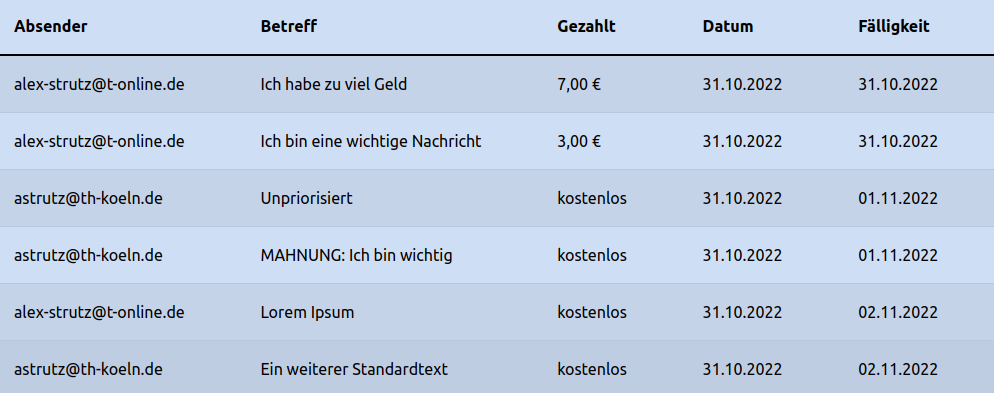
\includegraphics[width=1\textwidth]{Figures/inbox.png}
	\caption{Screenshot: Posteingang eines Empfängers, nach Priorität sortiert}
	\label{fig:screenshot_inbox}
\end{figure}

\noindent Mit Klick auf eine Tabellenzeile wird die entsprechende Nachricht in der Detailansicht \texttt{/receive/messages/:id} angezeigt. Anhand der ID wird die \texttt{Message} aus der Datenbank geladen und an das Frontend übergeben. Dieses zeigt die Nachricht, vergleichbar mit gängigen E-Mail Clients, in zweiteiliger Struktur aus Metadaten (E-Mail Header) und Inhalt (E-Mail Body) an. Anhang \ref{fig:screenshot_message} zeigt einen entsprechenden Screenshot. Zusätzlich wird ein \textit{Erledigt}-Button angezeigt, mit welchem ein Empfänger eine E-Mail als bearbeitet kennzeichnen kann. Dies ist jedoch nur bei E-Mails möglich, die am höchsten priorisiert sind. Bei Klick auf den Button wird die Action \texttt{messages\#destroy} aufgerufen. Die \texttt{Message} wird anhand des Query-Parameters ID geladen. Falls der Parameter \texttt{fetch} nicht gesetzt ist, es sich also nicht um einen Test handelt (vgl. \ref{Einsicht_in_das_E-Mail_Aufkommen}), wird der \texttt{EmailLoadJob} aufgerufen und die Nachricht mit \texttt{read\_message} gelesen. Dazu wird eine IMAP \texttt{SEARCH} ausgeführt, die die gefundene Nachricht als gelesen markiert. 

\begin{listing}[!ht]
\inputminted[firstline=8, lastline=17, linenos]{ruby}{Listings/Pkg3/messages_controller.rb}

\caption
    [Auszug: Erledigung einer Nachricht]
    {Auszug: Erledigung einer Nachricht durch Setzen eines Bearbeitungszeitpunktes (\texttt{app/controllers/receive/messages\_controller.rb})}

\label{lst:messages_controller}
\end{listing}

\noindent Darüber hinaus muss das System die Anzahl der erledigten Mails des \texttt{Recipient} je Tag vorhalten, um Aussagen über die noch zu erledigenden E-Mails tätigen zu können. Hierzu wird das Datenbankmodell der \texttt{Message} so erweitert, dass es einen Timestamp \texttt{processed\_at} enthält. Mit diesem Feld kann festgehalten werden ob und wann welche Nachricht erledigt wurde. Zusätzlich werden die Scopes \texttt{processed} und \texttt{unprocessed} implementiert. Scopes sind im Kontext von Ruby on Rails Datenbankselektionen, die auf Model-Ebene implementiert und daraufhin global mit \texttt{Model.scope} genutzt werden können \citep{Hansson2022c}. Im Falle der zuvor erwähnten Scopes führt \texttt{processed} die Query \texttt{where.not(processed\_at: nil)} und \texttt{unprocessed} die Query \texttt{where(processed\_at: nil)} aus. So können die bisherigen Views einfach angepasst werden, um nur unbearbeitete Nachrichten anzuzeigen. Die an einem Tag bearbeiteten E-Mails können im Scope \texttt{processed} mit einer Filterung nach dem Tag geladen werden. Sourcecode \ref{lst:messages_controller} zeigt die backendseitige Erledigung einer \texttt{Message}.

Mit dem implementierten Bearbeitungsdatum ist es nun möglich E-Mails für den Empfänger mit einem Fälligkeitsdatum zu versehen. Dazu wird beim Laden der Action \texttt{show} der \texttt{Inbox} die Funktion \texttt{calculate\_due\_dates} aufgerufen, siehe Sourcecode \ref{lst:inboxes_controller}. Diese Funktion erzeugt ein Array, welches die verschiedenen Fälligkeitsdaten enthält. Dazu wird eine Schleife durchlaufen. Für jede unbearbeitete Nachricht, nach Priorität sortiert, wird geprüft, ob ihr Index durch die Bearbeitungsleistung teilbar ist. Dabei werden die am heutigen Tag bearbeiteten E-Mails miteinbezogen. Ist der Rest der Division gleich 0, wird ein Tag zum Fälligkeitsdatum addiert. So entsteht ein Array an \texttt{DateTime}-Instanzen, das die gleiche Anzahl an Elementen wie die Liste an Nachrichten enthält. Das Array wird als Instanzvariable \texttt{@due\_dates} an die View übergeben, welche sie entsprechend in der Posteingangstabelle darstellt. 

\begin{listing}[!ht]
\inputminted[firstline=12, lastline=23, linenos]{ruby}{Listings/Pkg3/inboxes_controller.rb}

\caption
    [Auszug: Berechnung der Fälligkeitstermine]
    {Auszug: Berechnung der Fälligkeitstermine für Empfänger (\texttt{app/controllers/receive/inboxes\_controller.rb})}

\label{lst:inboxes_controller}
\end{listing}

\newpage

\noindent Zusätzlich zur Triage im Posteingang soll dem Empfänger die Möglichkeit gegeben werden Regeln zu definieren, nach welchen E-Mails die Triage überspringen und direkt bearbeitet werden können. Hierzu wird das Empfängerfrontend so erweitert, dass eine zweite Tabelle verfügbar ist, welche E-Mails enthält, auf welche die Regeln zutreffen. Diese E-Mails werden im Folgenden \textit{Ausnahmenachrichten} genannt. Die beiden Tabellen werden mit der \texttt{Tab}-Komponente von Bootstrap getrennt, sodass nur eine sichtbar ist und der Nutzer zwischen ihnen wechseln kann, siehe Anhang \ref{fig:screenshot_inbox2}. Der Posteingang listet weiterhin Ausnahmenachrichten auf, sodass der Empfänger sie regulär nach ihrer Fälligkeit bearbeiten kann, falls sie sich nach Sichtung als weniger relevant darstellen. Um zu ermitteln welche Nachrichten als Ausnahmenachrichten gelten, wird dem \texttt{Message}-Model ein weiterer Scope namens \texttt{matches\_rules} hinzugefügt, wie in Sourcecode \ref{lst:message3} zu sehen. Im Scope wird durch die Regeln des Posteingangs iteriert und für jede Regel eine Datenbankquery erzeugt, die nach Elementen sucht, die für das Feld definiert von \texttt{field\_to\_search} den Wert \texttt{field\_matcher} enthalten. Mögliche Werte für \texttt{field\_to\_search} sind \texttt{subject}, \texttt{sender\_address} oder \texttt{content}, die jeweils den Betreff, den Absender oder den Inhalt der E-Mail durchsuchen. Das Ergebnis der einzelnen Queries wird konkateniert und als Array, sortiert nach dem Versanddatum, zurückgegeben. Die Sortierung erfolgt bewusst nur nach dem Versanddatum und nicht nach dem Gegenwert, da dieser bei Ausnahmenachrichten nicht mehr relevant ist.

\begin{listing}[!ht]
\inputminted[firstline=6, lastline=15, linenos]{ruby}{Listings/Pkg3/message.rb}

\caption
    [Auszug: Scope zur Ermittlung der Ausnahmenachrichten]
    {Auszug: Scope zur Ermittlung der Ausnahmenachrichten für Empfänger (\texttt{app/models/message.rb})}

\label{lst:message3}
\end{listing}

\noindent Als letztes Feature wird das Anzeigen, Erstellen, Bearbeiten und Löschen (CRUD) von Regeln, sowie die Anpassung der Bearbeitungsleistung durch den Empfänger implementiert. Für Letztere werden dem \texttt{recipients\_controller} die Actions \texttt{edit} und \texttt{update} hinzugefügt. Dabei gibt \texttt{edit} ein Frontend zur Bearbeitung der Regeln, siehe Anhang \ref{fig:screenshot_recipients}, zurück. Bei Klick auf den Button wird die Action \texttt{update} aufgerufen, die den neuen Wert als \texttt{editing\_performance\_per\_day} speichert. Für die Regeln wurden entsprechende Views und Actions definiert, die dem bereits bekannten Schema folgen, benannt \texttt{new} und \texttt{create} zur Erstellung, \texttt{edit} und \texttt{update} zur Bearbeitung und \texttt{destroy} zum Löschen. Screenshots dieser Oberflächen finden sich in den Anhängen \ref{fig:screenshot_rules1} bis \ref{fig:screenshot_rules3}. Die Routenstruktur der finalen Anwendung ist in Anhang \ref{Routenstruktur_der_Anwendung} hierarchisch dargestellt.